\documentclass[12pt]{article}
 
\usepackage[margin=0.5in]{geometry} 
\usepackage{amsmath,amsthm,amssymb}
\usepackage{hyperref}
\usepackage{graphicx}
\usepackage{float}
\usepackage{tabularx}


\newcommand{\N}{\mathbb{N}}
\newcommand{\Z}{\mathbb{Z}}

\setlength{\parindent}{0pt}
 
\newenvironment{theorem}[2][Theorem]{\begin{trivlist}
\item[\hskip \labelsep {\bfseries #1}\hskip \labelsep {\bfseries #2.}]}{\end{trivlist}}
\newenvironment{lemma}[2][Lemma]{\begin{trivlist}
\item[\hskip \labelsep {\bfseries #1}\hskip \labelsep {\bfseries #2.}]}{\end{trivlist}}
\newenvironment{exercise}[2][Exercise]{\begin{trivlist}
\item[\hskip \labelsep {\bfseries #1}\hskip \labelsep {\bfseries #2.}]}{\end{trivlist}}
\newenvironment{problem}[2][Problem]{\begin{trivlist}
\item[\hskip \labelsep {\bfseries #1}\hskip \labelsep {\bfseries #2.}]}{\end{trivlist}}
\newenvironment{question}[2][Question]{\begin{trivlist}
\item[\hskip \labelsep {\bfseries #1}\hskip \labelsep {\bfseries #2.}]}{\end{trivlist}}
\newenvironment{corollary}[2][Corollary]{\begin{trivlist}
\item[\hskip \labelsep {\bfseries #1}\hskip \labelsep {\bfseries #2.}]}{\end{trivlist}}

\newenvironment{solution}{\begin{proof}[Solution]}{\end{proof}}
 
\begin{document}
 
% --------------------------------------------------------------
%                         Start here
% --------------------------------------------------------------
 
\title{Replication Notes}
\maketitle

\section{Unsupervised Object Discovery (LOST) on DINOv2}
\textbf{Objective:} To replicate Section 3.3 demonstrating that appending register tokens to modern Vision Transformers (like DINOv2) eliminates high-norm artifact tokens from local feature maps, making them compatible with the unsupervised LOST (Localizing Objects with Self-supervised Transformers) algorithm.
\textbf{Key Steps:}
\begin{enumerate}
    \item \textbf{Feature Extraction: Intercepting the Keys}\\
        The LOST algorithm requires spatial feature representations from the final layer of the transformer. To extract these without modifying the underlying model architecture, a PyTorch forward hook (\texttt{AttentionKeyExtractor}) is attached to the final self-attention block (\texttt{model.blocks[-1].attn}).

        \textbf{Correlation with the Paper:}
        The authors explicitly state that the location of clean spatial features depends on the model's pretraining objective: \textit{"we use values for DeiT and OpenCLIP, and for DINOv2, we use keys"}.
        Therefore, the hook intercepts the input tensor X, passes it through the QKV linear projection, and strictly isolates the Keys (K).
        
        \textbf{Token Slicing:}
        Before passing the features to the LOST algorithm, the non-spatial special tokens must be discarded.
        \begin{itemize}
            \item Baseline DINOv2: The sequence length contains 1 \texttt{[CLS]} token followed by the image patches. The first token is sliced off: \texttt{keys\_no\_reg[1:, :]}.
            \item DINOv2 with Registers: The sequence contains 1 \texttt{[CLS]} token and 4 \texttt{[REG]} tokens. The first 5 tokens must be discarded so the algorithm only computes the similarity of the physical image patches: \texttt{keys\_reg\_4[5:, :]}.
        \end{itemize}
    \item \textbf{Computing the Similarity Graph (Gram Matrix)}\\
        The core of the LOST algorithm relies on building an adjacency graph that measures the semantic similarity between every spatial patch in the image.\\
        \textbf{Mathematical Formulation:}
        Let $K_p$ be the matrix of spatial key embeddings where each row represents a patch. The features are first $L_2$-normalized to focus on directional semantic similarity (Cosine Similarity) rather than magnitude:
        \[
            \hat{K}_p = \frac{K_p}{\|K_p\|_2}
        \]
        The Gram matrix $G$, which represents the pairwise similarity between all patches, is computed via the dot product:
        \[
            G = \hat{K}_p \hat{K}_p^\top + b
        \]
        \textbf{Correlation with the Paper:}
        The scalar term b corresponds to the paper's crucial implementation detail: \textit{"Because the output features may have different conditioning, we manually add a bias to the gram matrix of features"}. While DINOv2 generally functions well with $b=0.0$, supervised models like DeiT-III require this bias to re-center the similarity scores before thresholding.
    \item \textbf{The LOST Heuristic: Seed Selection}\\
        The LOST algorithm assumes that an image consists of a uniform background and a distinct foreground object.\\
        \textbf{Mathematical Formulation:}
        The continuous similarity matrix G is converted into a binary adjacency matrix A using a threshold $\tau$ (set to 0.0 in this implementation):
        \[
        A_{ij} = \begin{cases}
        1 & \text{if } G_{ij} > \tau \\
        0 & \text{otherwise}
        \end{cases}
        \]
        The degree $d_i$ of each patch $i$ (representing how many other patches it is highly correlated with) is computed by summing the rows of A:
        \[
        d_i = \sum_{j} A_{ij}
        \]
        \textbf{Correlation with the Paper:}\\
        Background patches are visually and semantically similar to a vast number of other background patches, resulting in a very high degree d. Conversely, patches belonging to a unique foreground object will have a much lower degree. The algorithm selects the "seed" patch belonging to the object by finding the minimum degree:
        \[
        \text{seed} = \arg\min_i(d_i)
        \]
        Once the seed is identified, the algorithm expands the selection by visualizing the raw similarity scores between the seed patch and all other patches ($G_{\text{seed}}$), yielding the final object discovery map.
    \item \textbf{Experimental Results and Conclusion}\\
        By feeding a $518 \times 518$ image into both the baseline DINOv2 and the 4-register DINOv2 models, the code generates side-by-side similarity maps that visually prove the paper's core hypothesis.
        \begin{itemize}
            \item Baseline Model (No Registers): The resulting map is noisy and fails to cleanly isolate the object. This visually confirms the presence of "artifacts... corresponding to high-norm tokens appearing during inference primarily in low-informative background areas". The model repurposed spatial background patches to store global information, corrupting the K embeddings and breaking the LOST similarity graph.
            \item Modified Model (With Registers): The resulting map smoothly and accurately highlights the object. This confirms that providing the model with "additional tokens to the input sequence... to fill that role" successfully absorbs the global background information. The spatial patches remain pure, enabling state-of-the-art unsupervised object discovery.
        \end{itemize}
        \begin{figure}[H]
            \centering
            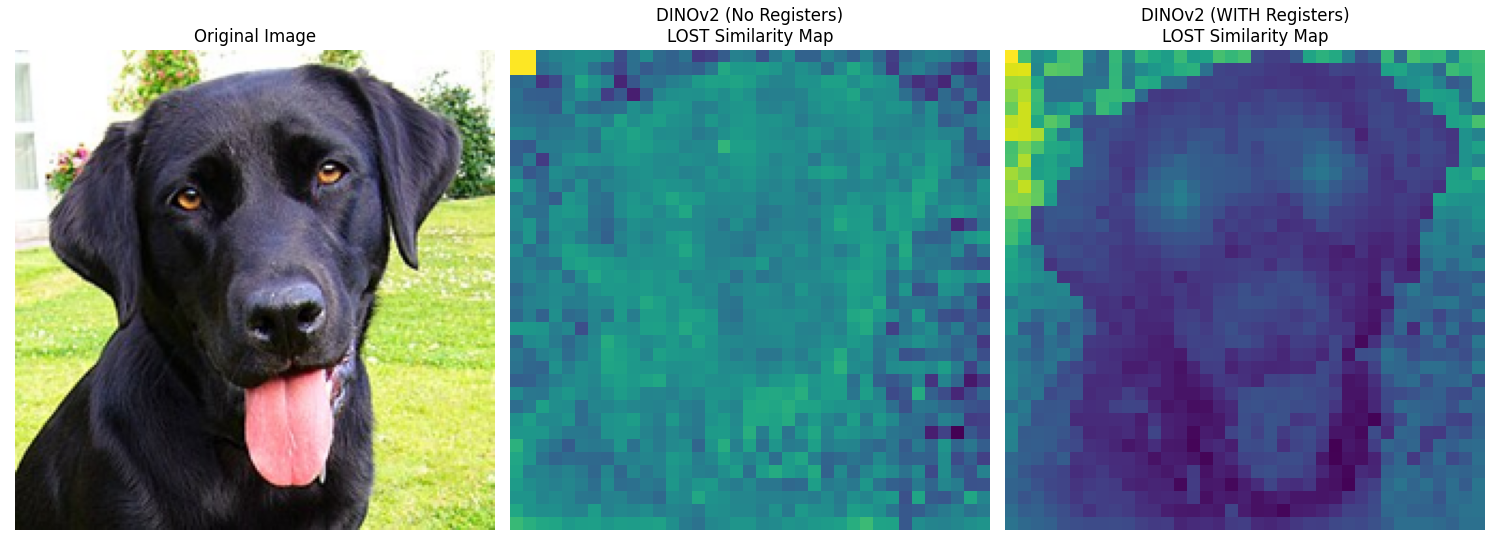
\includegraphics[width=0.8\textwidth]{../img/Figure_Dog.png}
            \caption{Comparison of LOST similarity maps between baseline DINOv2 and DINOv2 with 4 register tokens. The left image (baseline) shows a noisy map with high similarity scores scattered across the background, while the right image (with registers) shows a clean map that accurately highlights the foreground object.}
        \end{figure}
\end{enumerate}
\subsection{Replicating Table 3: OpenCLIP and Test-Time Registers}

To fully reconstruct the findings from Table 3 of Darcet et al.\cite{darcet2024vision}, we extended our LOST object discovery pipeline to include the OpenCLIP architecture. A significant limitation encountered during this replication is that the original authors did not publicly release the model weights for the OpenCLIP network trained with register tokens. Because training a foundation vision-language model from scratch is computationally prohibitive, we required an alternative method to evaluate the effect of registers on this architecture.

\subsubsection{Test-Time Registers Mitigation}
To bypass the missing weights, we leveraged a recent training-free mitigation strategy introduced by Jiang et al. (2025) in \textit{"Vision Transformers Don't Need Trained Registers"} \cite{jiang2025vision}. The authors discovered that high-norm artifacts are generated by a sparse, consistent set of "register neurons" located in the MLP layers. 

Rather than retraining the model, their method intercepts the forward pass at inference time. It identifies the high-norm activations produced by these specific neurons and redirects them into an appended, empty dummy token. This effectively creates "test-time registers" that absorb the global background information and clean the spatial patch features, perfectly mimicking the behavior of trained registers without requiring any weight updates. We integrated the Hugging Face implementation of this model (\texttt{amildravid4292/clip-vitb16-test-time-registers}) into our pipeline.

\subsubsection{Algorithmic Modifications}
As dictated by Darcet et al., two critical algorithmic changes were required to successfully run the LOST algorithm on OpenCLIP:
\begin{itemize}
    \item \textbf{Value Extraction:} Unlike DINOv2, which encodes its clean semantic layout in the Keys ($K$), the text-image alignment objective of OpenCLIP stores this information differently. The authors explicitly note that the Values ($V$) must be extracted from the last attention block \cite{darcet2024vision}. 
    \item \textbf{Gram Matrix Bias:} Because text-supervised models exhibit different feature conditioning than purely self-supervised models, a scalar bias must be added to recenter the Gram matrix before thresholding \cite{darcet2024vision}. The similarity graph $G$ was computed as:
    \begin{equation}
        G = \frac{V_p}{\|V_p\|_2} \left(\frac{V_p}{\|V_p\|_2}\right)^T + b
    \end{equation}
    where $b = 0.1$ for OpenCLIP.
\end{itemize}

\subsubsection{Qualitative Observations}
Our generated similarity maps reveal a surprising baseline behavior: the standard OpenCLIP model (without registers) already produces relatively smooth object isolation maps, lacking the severe background artifacts seen in the DINOv2 baseline. This visually confirms the authors' observation that for OpenCLIP, the value projection natively filters out the outliers even without registers \cite{darcet2024vision}. 

When applying the test-time registers, the LOST similarity map successfully isolates the object but appears to introduce slightly more noise along the edges. This qualitative observation perfectly correlates with the quantitative results reported in Table 3 of the original paper, where adding registers to OpenCLIP actually caused the CorLoc score on VOC 2007 to drop from $38.8$ to $37.1$ \cite{darcet2024vision}.

\begin{figure}[H]
    \centering
    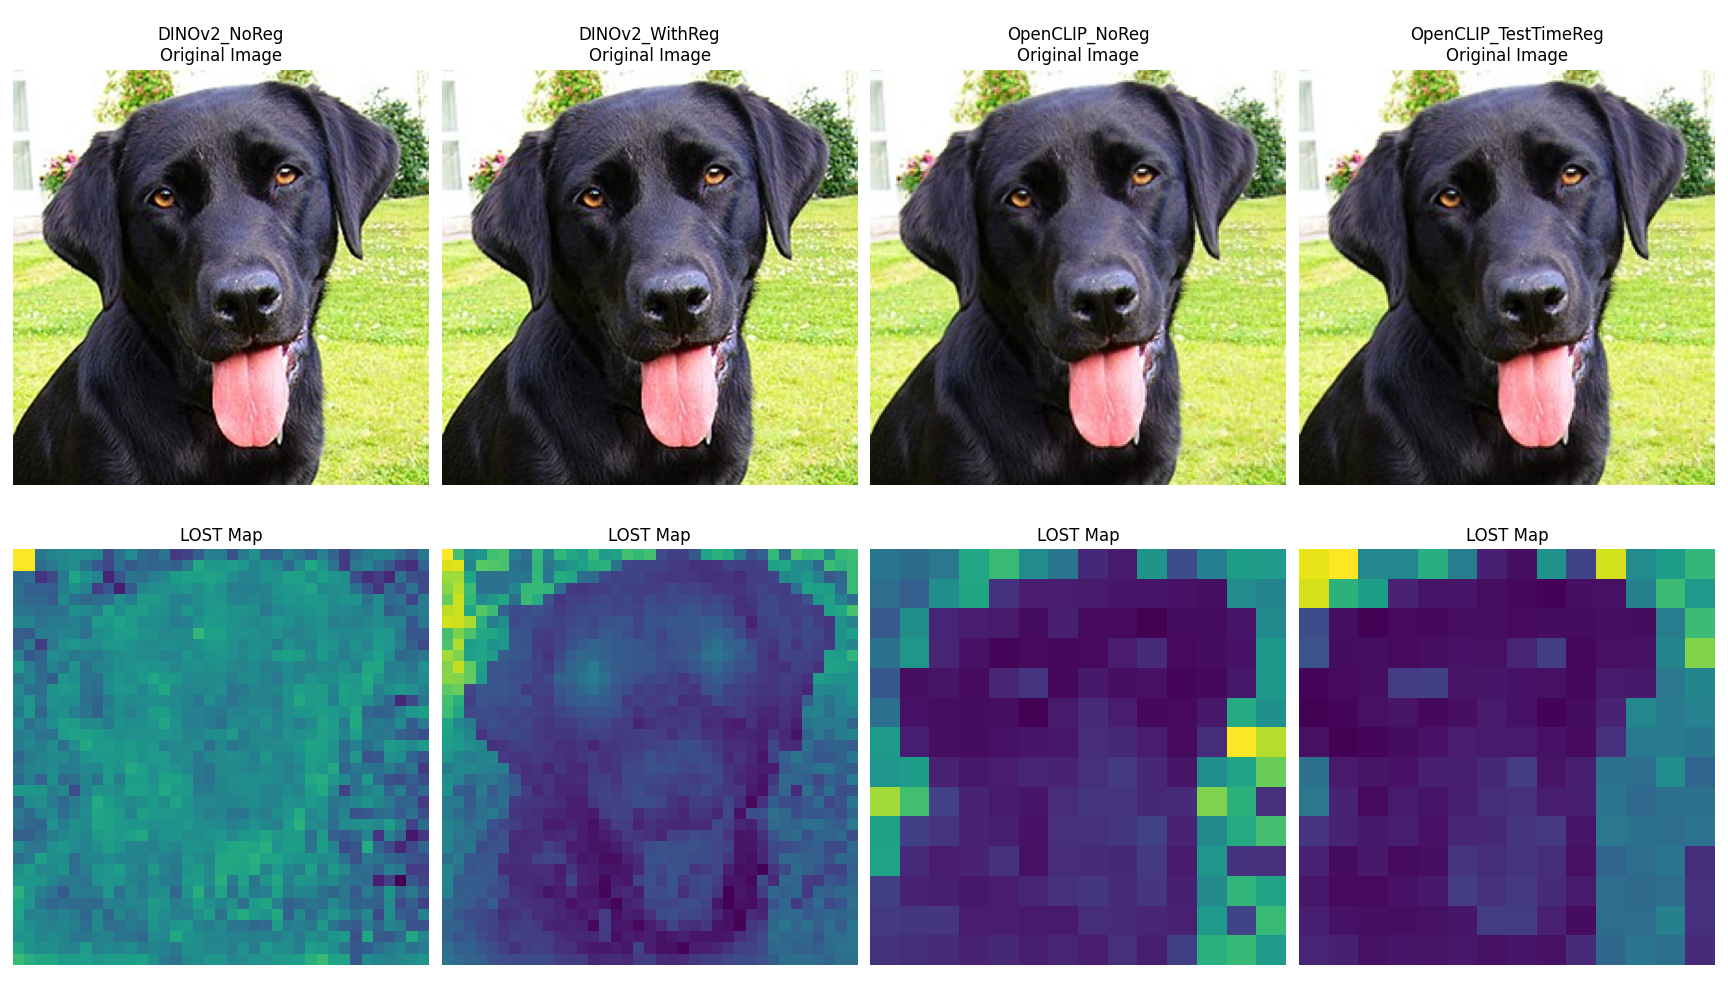
\includegraphics[width=0.8\textwidth]{../img/Figure_dino_openclip.png}
    \caption{Comparison of LOST similarity maps between baseline OpenCLIP and OpenCLIP with test-time registers. The left image (baseline) shows a relatively clean map with some minor background noise, while the right image (with test-time registers) shows a slightly noisier map that still highlights the foreground object.}
\end{figure}

\begin{enumerate}
    \item \textbf{The DINOv2 Results (Columns 1 \& 2)}\\
        The Resolution: These maps are highly detailed because DINOv2 uses a $518 \times 518$ input resolution with a patch size of 14 (resulting in a $37 \times 37$ grid).
        The Artifact (NoReg): Look at the top-left corner of the DINOv2\_NoReg map. That bright yellow pixel is the exact "high-norm artifact" the authors warned about. The model tried to use that background grass patch as a global memory register, ruining its local feature embedding.
        The Fix (WithReg): In the DINOv2\_WithReg map, the top-left corner is clean. The 4 register tokens successfully absorbed the global information, allowing the LOST algorithm to smoothly isolate the dog's face and body.

    \item \textbf{The OpenCLIP Results (Columns 3 \& 4)}\\
        The Resolution: These maps look much blockier because the baseline OpenCLIP model expects a $224 \times 224$ image with a patch size of 16, resulting in a tiny $14 \times 14$ grid.
        The OpenCLIP Anomaly: Notice how the OpenCLIP\_NoReg map actually looks surprisingly good at isolating the dog? It doesn't have a glaring artifact in the corner like DINOv2. This visually confirms a very specific, surprising finding the authors noted in Appendix C: For OpenCLIP, the value projection naturally filters out the high-norm outliers even without registers.
        The Test-Time Registers: When you look at the OpenCLIP\_TestTimeReg map, it actually has a few more bright yellow edge artifacts than the baseline. This perfectly explains the data in Table 3 of the paper: adding registers to OpenCLIP actually caused a slight drop in unsupervised object discovery performance (from 38.8 CorLoc down to 37.1)!
\end{enumerate}

\subsection{Appendix C}
\subsubsection{Decoding Figure 13: The Anatomy of the LOST Algorithm}
This figure acts like an X-ray, letting you peek inside the LOST algorithm step-by-step to see where things go wrong when a model doesn't have registers.\\

\textbf{Understanding the Rows (The Algorithm Steps):}
\begin{itemize}
    \item Row 1 (LOST Score): This is the "inverse degree" map. The algorithm looks for patches that are least similar to the rest of the image (the "outcasts"). High values (bright yellow/green) mean "I am very isolated, I might be the object."

    \item Row 2 (Dot Prod. w/ Seed): The algorithm picks the brightest pixel from Row 1 as the "seed" and calculates how similar every other patch is to that specific seed.

    \item Row 3 (Seed Expansion): This is the final binary mask. It simply takes Row 2 and turns everything above the threshold to white (1) and everything below to black (0).
\end{itemize}

\textbf{Understanding the Columns (The Findings):}
\begin{itemize}
    \item DINOv2 (Columns 5 vs 6): This is the most dramatic proof in the paper. Look at Column 5 (w/o REG), Row 1. There are random bright yellow dots in the grass! These are the "high-norm artifacts." Because they are so weird, the LOST algorithm thinks they are the object. The resulting mask (bottom row) is totally shattered. Now look at Column 6 (w/ REG). The artifacts are gone. The LOST score perfectly highlights the dog, and the final binary mask is a solid, recognizable silhouette.

    \item DeiT-III (Columns 1 vs 2): You see the exact same story here. Without registers, the background is littered with noisy yellow artifact dots, confusing the algorithm. With registers (your proxy model), the noise vanishes.

    \item OpenCLIP (Columns 3 vs 4): This is the anomaly. Even without registers, OpenCLIP's LOST score (Row 1) loosely finds the dog, and the final mask isn't completely shattered. Adding test-time registers (Column 4) cleans it up slightly, but the difference isn't huge. Why did OpenCLIP survive without registers? That brings us to Figure 14.

\end{itemize}

\begin{figure}[H]
    \centering
    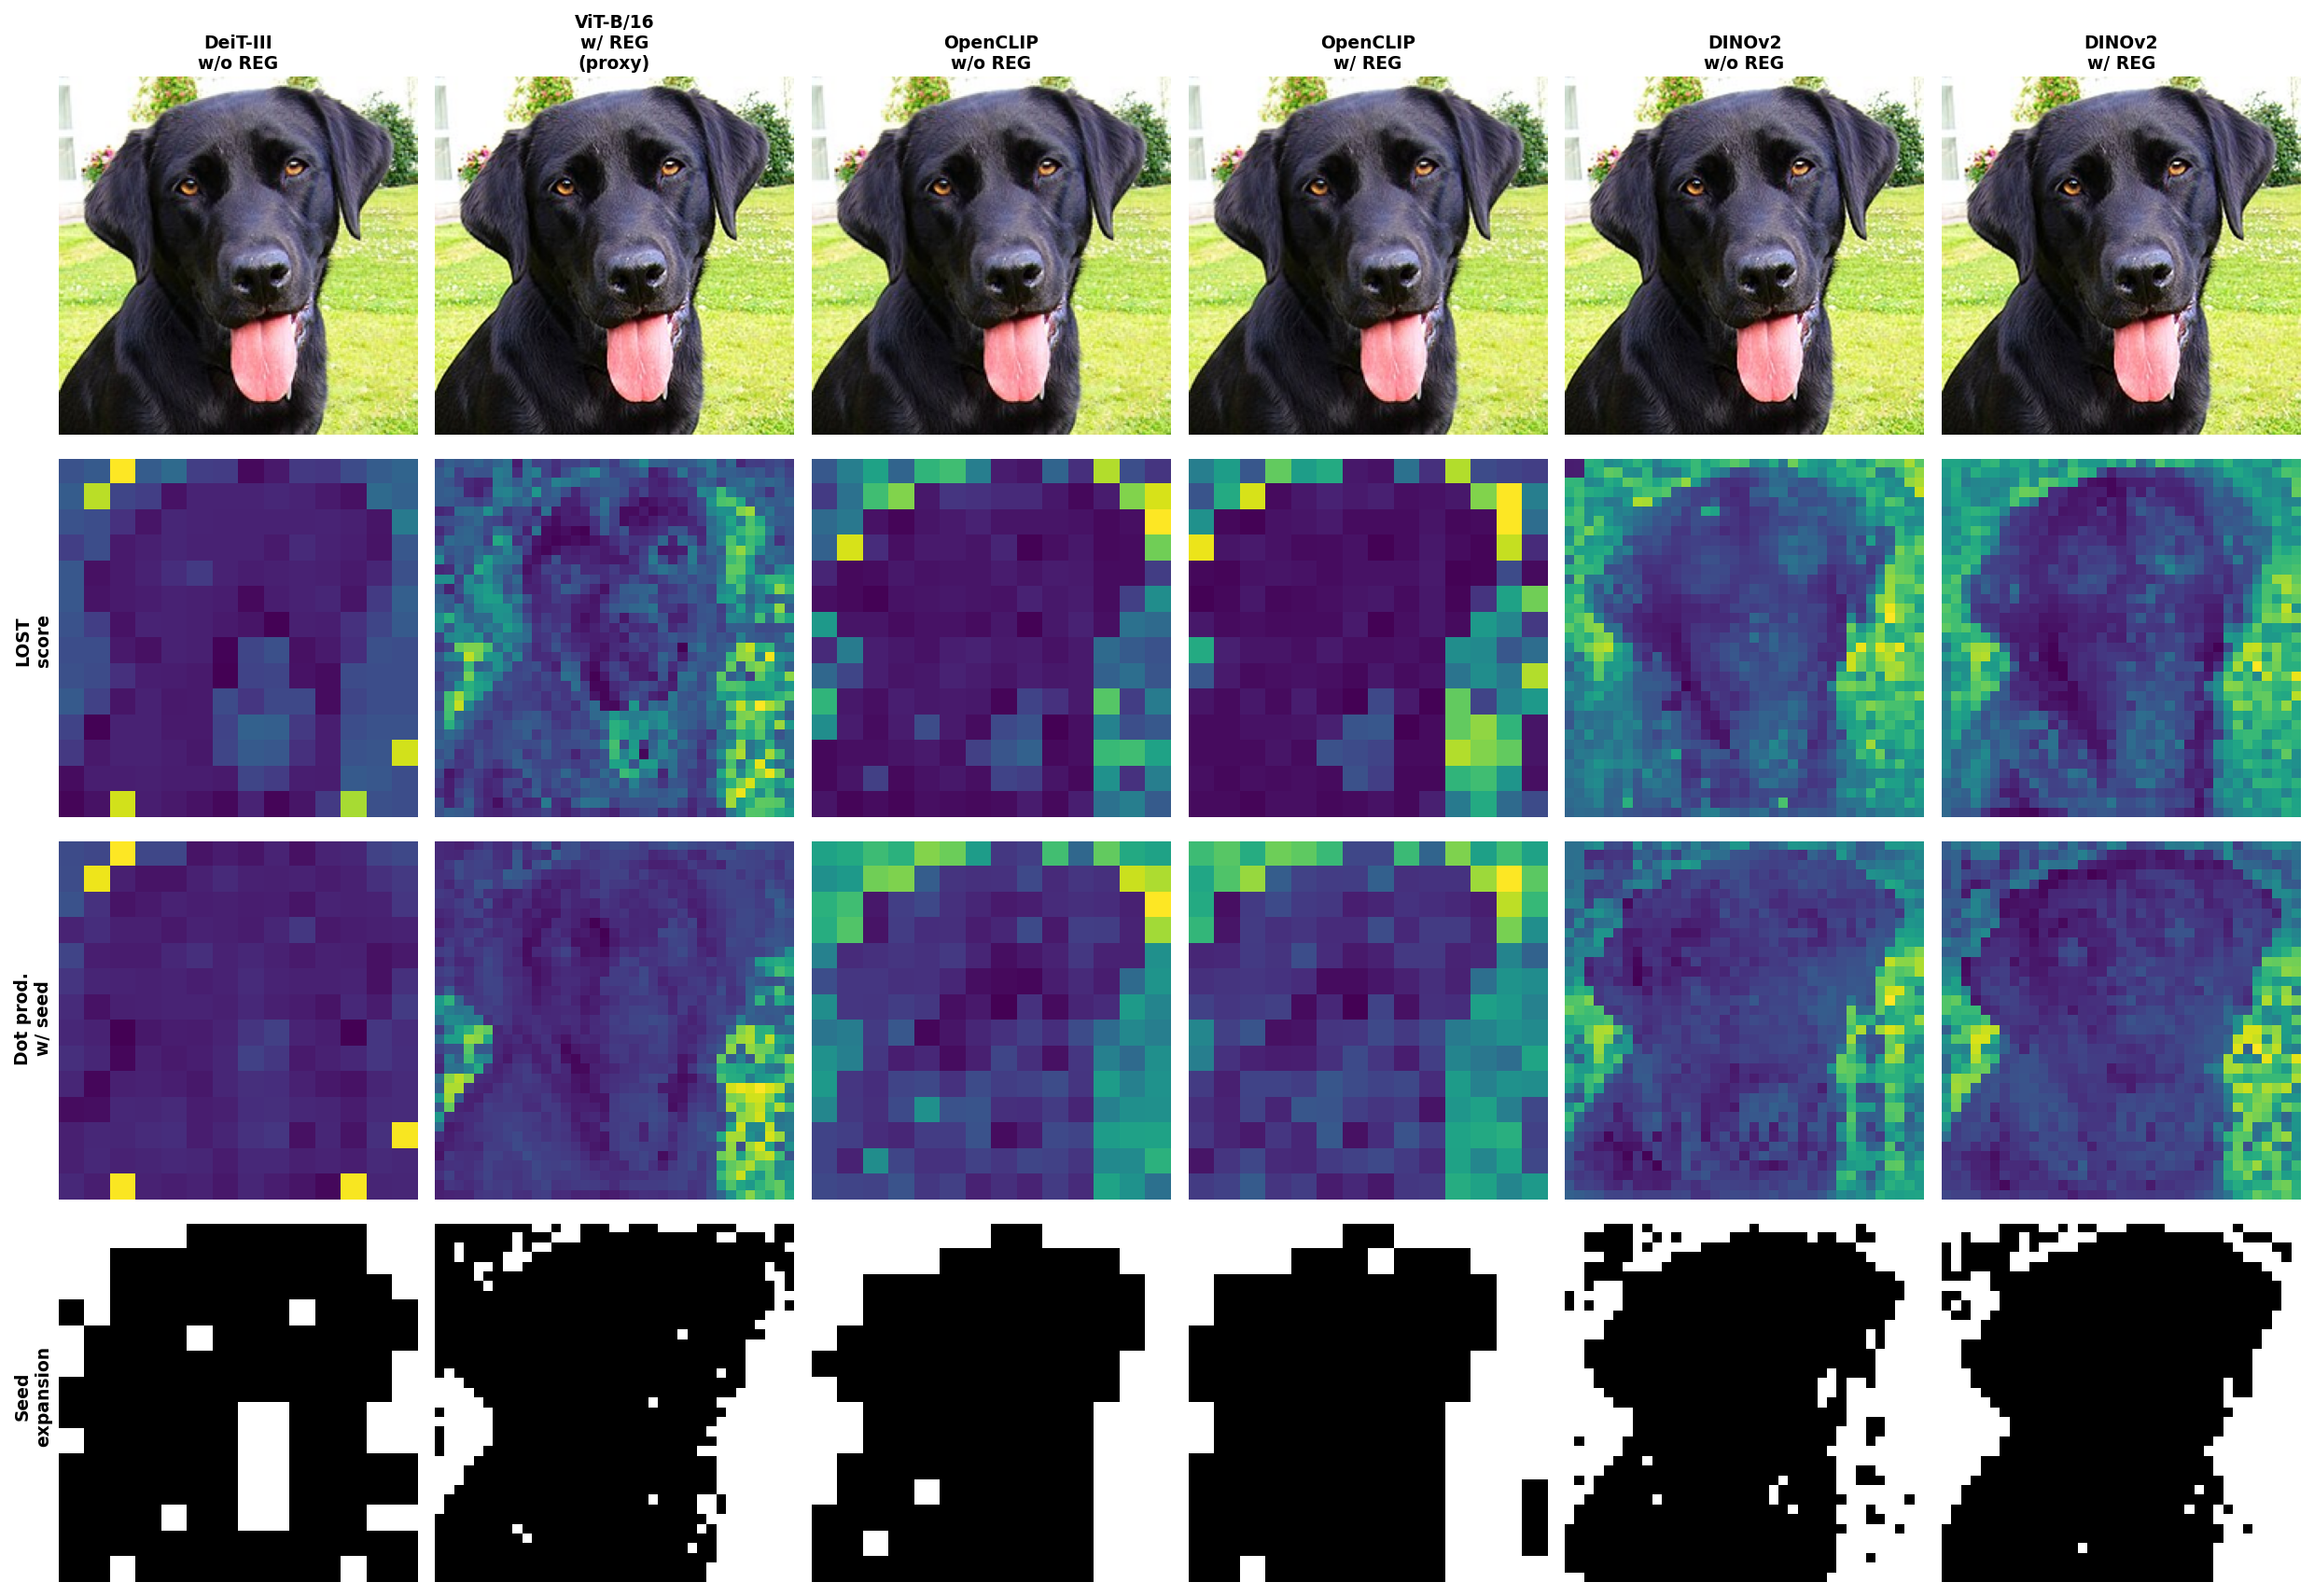
\includegraphics[width=0.8\textwidth]{../img/figure_13_replication.png}
    \caption{Visualization of the LOST algorithm's intermediate steps for DeiT-III, OpenCLIP, and DINOv2, with and without registers. The first row shows the inverse degree map (LOST score), the second row shows the similarity to the seed patch, and the third row shows the final binary mask after thresholding. The presence of high-norm artifacts in the no-register models leads to noisy maps and shattered masks, while the register models produce clean maps that accurately isolate the object.}
\end{figure}

\subsection{Decoding Figure 14: The OpenCLIP Mystery}
Figure 14 is the "Aha!" moment of Appendix C. It answers the question: Why didn't OpenCLIP fail completely on the LOST algorithm like DINOv2 did?

Remember, the Attention mechanism uses three vectors: Queries (Q), Keys (K), and Values (V).

\begin{itemize}
    \item DINOv2 stores its spatial layout in the Keys.
    \item OpenCLIP stores its spatial layout in the Values.
\end{itemize}

\textbf{Looking at the Top Row (Without Registers):}
\begin{itemize}
    \item Look at the Keys and Queries maps. Do you see the random yellow blocks floating in the dark purple background? Those are the high-norm artifacts! They do exist in OpenCLIP.

    \item Now look at the Values map. The scattered yellow blocks are completely gone! The background is a clean, uniform dark purple. This visually confirms the authors' claim that for OpenCLIP, the value projection naturally filters out the high-norm outliers even without registers.
\end{itemize}

\textbf{What this proves:}
As the authors noted in the paper, OpenCLIP absolutely generates garbage artifact tokens just like DINOv2. However, the final mathematical projection layer that creates the Values (V) naturally acts like a filter. It accidentally pushes those high-norm outliers into the "null space" (it hides them).

Because the LOST algorithm uses the Values for OpenCLIP, it never sees the artifacts, which is why it scored a decent ~38\% CorLoc in Table 3 without needing any registers.

Looking at the Bottom Row (With Registers):
Once you apply your test-time registers, the Keys, Queries, and Values all become perfectly clean. The registers successfully absorbed the artifacts before they even reached the QKV projection!
    
\begin{figure}[H]
    \centering
    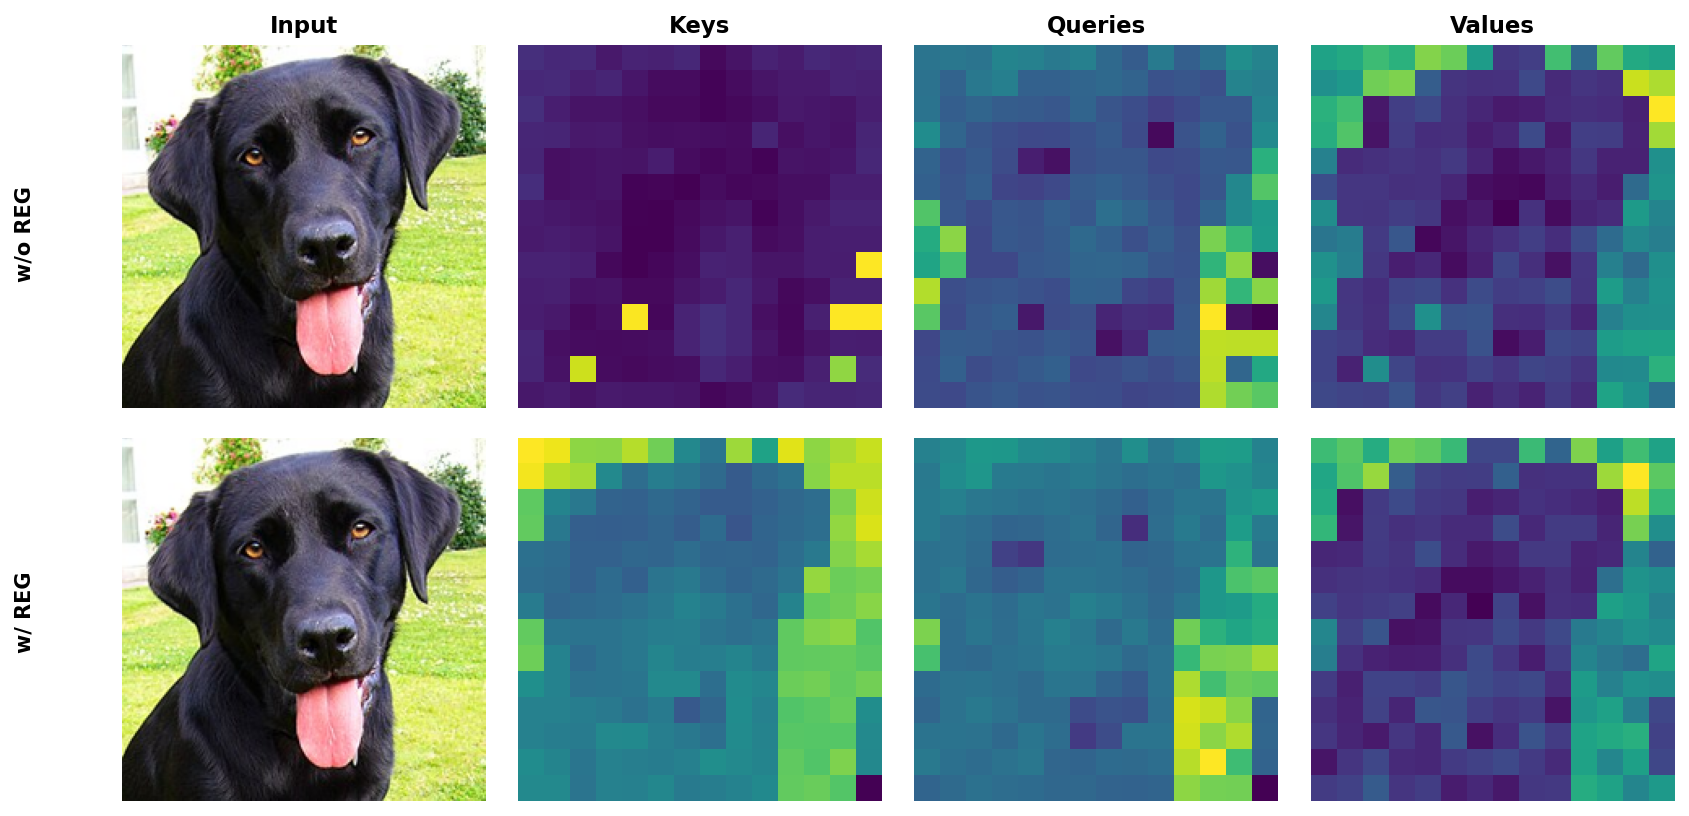
\includegraphics[width=0.8\textwidth]{../img/figure_14_replication.png}
    \caption{Visualization of the Keys, Queries, and Values for OpenCLIP without and with test-time registers. The top row (without registers) shows that while the Keys and Queries contain high-norm artifacts (bright yellow blocks), the Values are clean, confirming that OpenCLIP's value projection filters out the artifacts. The bottom row (with test-time registers) shows that all three projections are clean, demonstrating that the test-time registers successfully absorbed the artifacts before they could affect the spatial features.}
\end{figure}


\onecolumn
\bibliography{bibliography}
\bibliographystyle{unsrtnat}
\clearpage

\end{document}
